\documentclass[11pt,a4paper]{article}
\usepackage{fontspec}
\setmainfont[Path=fonts/,FontIndex=7,BoldFont=AvenirNext.ttc,BoldFeatures={FontIndex=2},ItalicFont=AvenirNext.ttc,ItalicFeatures={FontIndex=4},BoldItalicFont=AvenirNext.ttc,BoldItalicFeatures={FontIndex=3}]{AvenirNext.ttc}
\setsansfont[Path=fonts/,FontIndex=7,BoldFont=AvenirNext.ttc,BoldFeatures={FontIndex=2},ItalicFont=AvenirNext.ttc,ItalicFeatures={FontIndex=4},BoldItalicFont=AvenirNext.ttc,BoldItalicFeatures={FontIndex=3}]{AvenirNext.ttc}
\newfontfamily\heavy[Path=fonts/,FontIndex=2]{AvenirNext.ttc}
\setmonofont[Path=fonts/,BoldFont=JetBrainsMono-Bold.ttf,ItalicFont=JetBrainsMono-Italic.ttf,Contextuals=NoAlternate,Ligatures=NoCommon]{JetBrainsMono-Regular.ttf}
\usepackage{xcolor,graphicx,tikz,booktabs,tabularx,listings,amsmath}
\usetikzlibrary{arrows.meta,positioning}
\definecolor{paper}{HTML}{FFFFFF}
\definecolor{ink}{HTML}{252525}
\definecolor{teal}{HTML}{252525}
\definecolor{orange}{HTML}{777777}
\definecolor{wash}{HTML}{EAEAEA}
\definecolor{quiet}{HTML}{666666}
\definecolor{lightink}{HTML}{D0D0D0}
\definecolor{codepaper}{HTML}{F6F6F4}
\lstset{language=Python,basicstyle=\ttfamily\fontsize{9.5}{13}\selectfont\color{ink},keywordstyle=\bfseries\color{ink},commentstyle=\itshape\color{quiet},stringstyle=\color{ink},showstringspaces=false,columns=fullflexible,keepspaces=true,breaklines=true,breakatwhitespace=true,numbers=none,upquote=true,aboveskip=8pt,belowskip=6pt}
\hyphenpenalty=4000
\emergencystretch=3em
% The same two-line navigation and fine rule as the reference, without a candy motif.
\newcommand{\guideheader}[2]{\begin{tikzpicture}[remember picture,overlay]
\node[anchor=north west,inner sep=0,text width=176mm] at ([xshift=16mm,yshift=-7mm]current page.north west) {\fontsize{8.5}{10}\selectfont\color{quiet}#1};
\node[anchor=north west,inner sep=0,text width=176mm] at ([xshift=16mm,yshift=-11.5mm]current page.north west) {\heavy\fontsize{10}{12}\selectfont\color{ink}#2};
\draw[lightink,line width=.4pt] ([xshift=16mm,yshift=-17mm]current page.north west)--([xshift=192mm,yshift=-17mm]current page.north west);
\end{tikzpicture}}

\usepackage[a4paper,left=16mm,right=18mm,top=24mm,bottom=19mm,headheight=14pt]{geometry}
\usepackage{fancyhdr,enumitem,hyperref}
\hypersetup{colorlinks=true,linkcolor=teal,urlcolor=teal}
\setlength{\parindent}{0pt}
\setlength{\parskip}{7pt}
\setlist{nosep,leftmargin=1.4em}
\usepackage{needspace,colortbl}
\lstdefinestyle{numbered}{numbers=left,numberstyle=\ttfamily\fontsize{7.5}{13}\selectfont\color{lightink},numbersep=10pt,xleftmargin=24pt}
\pagestyle{fancy}\fancyhf{}
\fancyhead[C]{\guideheader{Lesson 1 · Staircase and Frog}{Worksheet Answers · \nouppercase{\leftmark}}}
\fancyfoot[L]{\fontsize{8}{10}\selectfont\color{quiet}LESSON 1 / Staircase and Frog}
\fancyfoot[R]{\fontsize{9}{11}\selectfont\color{quiet}\thepage}
\renewcommand{\headrulewidth}{0pt}
\newcommand{\topic}[2]{\clearpage\markboth{#2}{}{\color{quiet}\fontsize{9}{12}\selectfont\textbf{#1}}\par{\heavy\fontsize{19}{23}\selectfont\raggedright #2\par}\vspace{5pt}}
\newcommand{\topicflow}[2]{\par\Needspace{20\baselineskip}\bigskip\markboth{#2}{}{\color{quiet}\fontsize{9}{12}\selectfont\textbf{#1}}\par{\heavy\fontsize{19}{23}\selectfont\raggedright #2\par}\vspace{5pt}}
\newcommand{\labeltext}[1]{{\color{teal}\textbf{#1}}\par}
\makeatletter
\newsavebox{\qbox}
\newenvironment{qblock}[1][0.6]{\def\qlimit{#1}\par\setbox\qbox\vbox\bgroup\hsize\linewidth\color@begingroup}{\par\color@endgroup\egroup
  \ifdim\dimexpr\ht\qbox+\dp\qbox\relax>\qlimit\textheight\relax\unvbox\qbox\else\box\qbox\fi\par}
\makeatother
\newcommand{\qtopic}[2]{{\color{quiet}\fontsize{9}{12}\selectfont\textbf{#1}}\par{\heavy\fontsize{19}{23}\selectfont\raggedright #2\par}\vspace{5pt}}
\begin{document}\color{ink}\fontsize{10.5}{13}\selectfont
\thispagestyle{empty}\pagecolor{white}\null
\begin{tikzpicture}[remember picture,overlay]
\node[anchor=north west,inner sep=0,text width=174mm] at ([xshift=18mm,yshift=-22mm]current page.north west)
{\heavy\fontsize{9}{12}\selectfont ALGORITHMS\quad /\quad LESSON 01\quad /\quad WORKSHEET ANSWERS};
\node[anchor=north west,inner sep=0,text width=174mm] at ([xshift=18mm,yshift=-39mm]current page.north west)
{\heavy\fontsize{43}{47}\selectfont\raggedright\spaceskip=.25em Staircase\\and Frog\par};
\node[anchor=north west,inner sep=0,text width=174mm] at ([xshift=18mm,yshift=-80mm]current page.north west)
{\fontsize{19}{25}\selectfont Worked answers, tables and complete code.};
\node[anchor=north west,inner sep=0,text width=150mm] at ([xshift=18mm,yshift=-97mm]current page.north west)
{\fontsize{12}{16}\selectfont Check each answer against your own working.\\Follow the question IDs from the worksheet.};
\node[anchor=center,inner sep=0] at ([xshift=105mm,yshift=-167mm]current page.north west)
{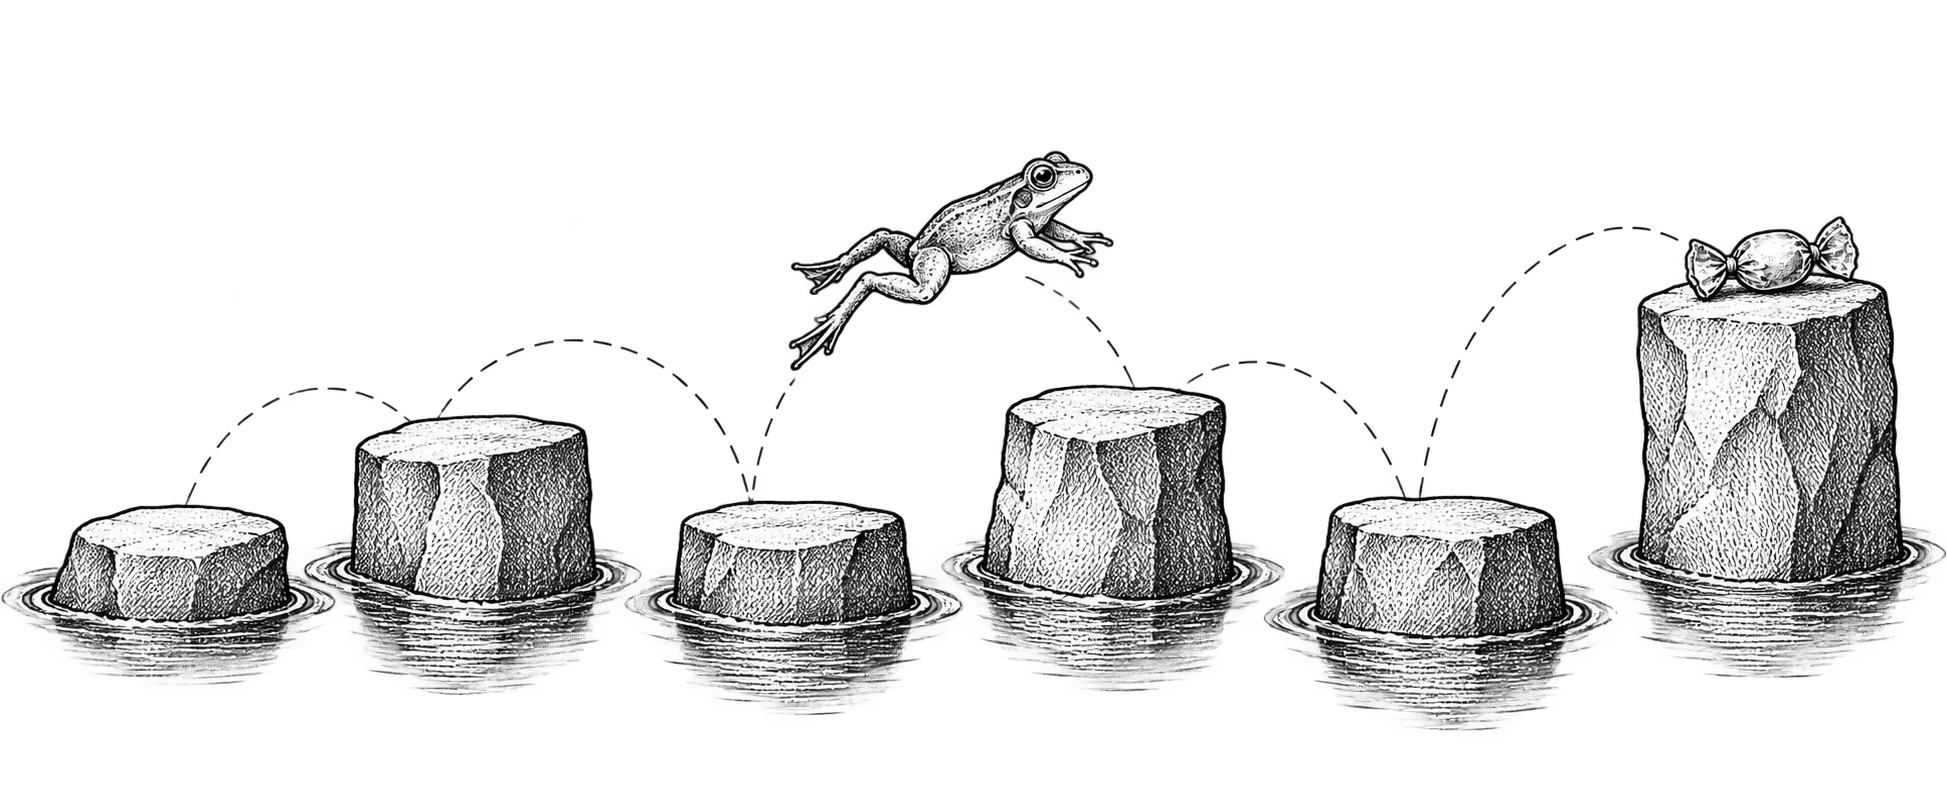
\includegraphics[width=174mm,height=94mm,keepaspectratio]{assets/cover.png}};
\node[anchor=north west,inner sep=0,text width=174mm] at ([xshift=18mm,yshift=-224mm]current page.north west)
{\fontsize{12}{16}\selectfont Questions appear in worksheet order.\\Alternative correct solutions are welcome.};
\node[anchor=west,inner sep=0] at ([xshift=18mm,yshift=-269mm]current page.north west)
{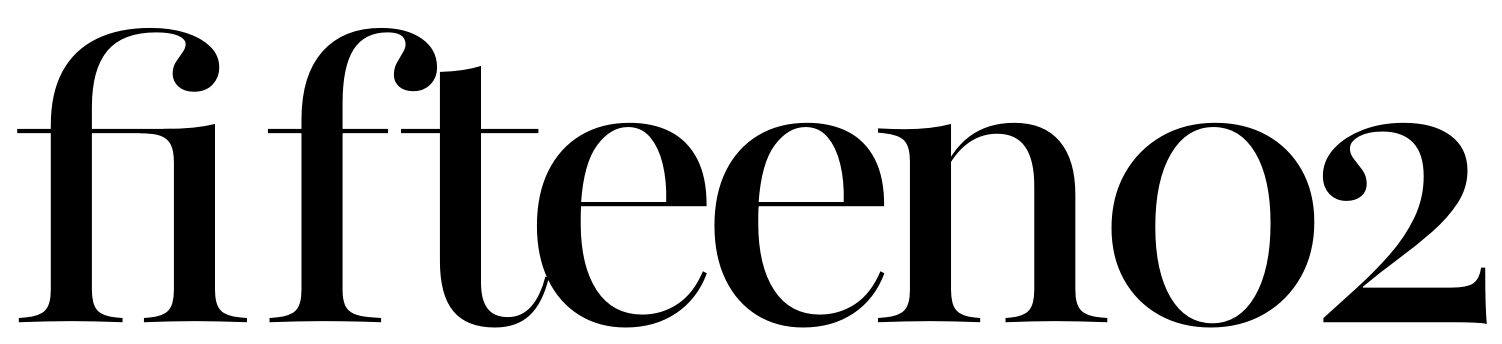
\includegraphics[width=43mm]{assets/logo.png}};
\node[anchor=east,inner sep=0] at ([xshift=192mm,yshift=-269mm]current page.north west)
{
\includegraphics[width=62mm]{assets/julians-pathfinder-monochrome.pdf}};
\end{tikzpicture}\clearpage
\topic{KEEP BESIDE YOUR WORK}{The route and the rules}
\textbf{Our route}\par Start with a brief recursion refresher; choose one warm-up exercise if you already know how calls stop. Then count staircase routes by hand. Write a recursive function, see which questions repeat, and save their answers. Then fill the same answers with a loop. Change the allowed jumps before trying Frog, where the answer is a minimum cost instead of a count.\par\medskip
\textbf{Recursion warm-up · L1-01 to L1-04}\par A function may call itself on a smaller input. The base case answers directly, without another call; every other call must move closer to the base case. A call that is waiting for a smaller call stays unfinished until that call returns its value.\par\medskip
\textbf{Staircase rules · L1-05 to L1-13}\par Start at ground level, called step 0. A move climbs exactly 1 or 2 steps. Count ordered lists of moves that land exactly on the target. For example, [1, 2] and [2, 1] are different routes. In L1-13 only, the permitted moves change to 1 or 3.\par\medskip
\textbf{Frog rules · L1-14 to L1-20}\par Number the stones 0, 1, 2 and so on. Start on stone 0 and finish on the last stone. A jump moves forward by one or two stone positions. Its cost is the absolute height difference: a jump from height 50 to height 30 costs 20. Add every jump cost in a route; find the smallest total.\par\medskip
\textbf{Names used in the questions}\par \texttt{ways(n)} is a function returning the number of staircase routes to target step n. \texttt{ways[n]} is a list entry storing that count. Parentheses call a function; square brackets read a stored entry. In Frog, \texttt{heights[i]} is the height at stone position i, while \texttt{best[i]} is the cheapest total cost to reach it.\par\medskip
\textbf{What to complete in class}\par Complete both staircase and Frog: for each, follow the slow recursive solution, save repeated answers, then fill a table with a loop. The recursion warm-up is a short refresher; the remaining warm-up exercises can be used for extra practice. Explain each small example before running a large input.\par\medskip
\textbf{Using these answers.} Each question and its supplied diagram or table appear before the answer. Completed tables, and answer diagrams where the question has one, follow the worked answer. The IDs match the worksheet; answer pages have their own page numbers. Each program is printed in full once, with imports, line numbers and a small check; a later question that uses the same program names the page where it appears and gives its own check. An optional question remains optional here.\par\bigskip{\color{lightink}\hrule height .4pt}\bigskip\par\markboth{A function that calls itself}{}\begin{qblock}\begin{qblock}[0.95]
\qtopic{L1-01}{A function that calls itself}
{\small\color{quiet}Warm-up: functions that call themselves}\par\medskip
\textbf{Question.} A function may call itself on a smaller input. countdown(n) below prints n and then calls countdown(n - 1); when n is 0 it prints Go! and makes no further call. In the table, write every call that countdown(3) makes, in order, what that call prints and which call it makes next.

\textbf{Code supplied with the question.}
\begin{lstlisting}
def countdown(n):
    if n == 0:
        print('Go!')
        return
    print(n)
    countdown(n - 1)
\end{lstlisting}
\textbf{Table supplied with the question.}\par\par\medskip \begingroup\small\setlength{\tabcolsep}{4pt}\renewcommand{\arraystretch}{1.35}\begin{tabularx}{\linewidth}{>{\raggedright\arraybackslash}X>{\raggedright\arraybackslash}X>{\raggedright\arraybackslash}X}\toprule\textbf{Call} & \textbf{Prints} & \textbf{Calls next}\\\midrule
countdown(3) &  & \\
 &  & \\
 &  & \\
 &  & \\
\bottomrule\end{tabularx}\endgroup\par\medskip 
\par\medskip\textbf{Worked answer.} Read the completed table from top to bottom. Each call prints before making the next call; the base case makes no further call.

\textbf{Completed table.}\par\par\medskip \begingroup\small\setlength{\tabcolsep}{4pt}\renewcommand{\arraystretch}{1.35}\begin{tabularx}{\linewidth}{>{\raggedright\arraybackslash}X>{\raggedright\arraybackslash}X>{\raggedright\arraybackslash}X}\toprule\textbf{Call} & \textbf{Prints} & \textbf{Calls next}\\\midrule
countdown(3) & 3 & countdown(2)\\
countdown(2) & 2 & countdown(1)\\
countdown(1) & 1 & countdown(0)\\
countdown(0) & Go! & nothing\\
\bottomrule\end{tabularx}\endgroup\par\medskip 
\end{qblock}
\end{qblock}\par\medskip{\color{lightink}\hrule height .4pt}\bigskip
\par\markboth{Wait for the smaller answer}{}\begin{qblock}\begin{qblock}[0.95]
\qtopic{L1-02}{Wait for the smaller answer}
{\small\color{quiet}Warm-up: functions that call themselves}\par\medskip
\textbf{Question.} sum\_squares(n) returns 0 when n is 0; otherwise it returns n * n + sum\_squares(n - 1). A call cannot finish until the call it waits for has returned. Fill the table for sum\_squares(4), starting from the bottom row and working up. Write the addition for each returned value.

\textbf{Code supplied with the question.}
\begin{lstlisting}
def sum_squares(n):
    if n == 0:
        return 0
    return n * n + sum_squares(n - 1)
\end{lstlisting}
\textbf{Table supplied with the question.}\par\par\medskip \begingroup\small\setlength{\tabcolsep}{4pt}\renewcommand{\arraystretch}{1.35}\begin{tabularx}{\linewidth}{>{\raggedright\arraybackslash}X>{\raggedright\arraybackslash}X>{\raggedright\arraybackslash}X}\toprule\textbf{Call} & \textbf{Waits for} & \textbf{Returns}\\\midrule
sum\_squares(4) &  & \\
sum\_squares(3) &  & \\
sum\_squares(2) &  & \\
sum\_squares(1) &  & \\
sum\_squares(0) & nothing & 0\\
\bottomrule\end{tabularx}\endgroup\par\medskip 
\par\medskip\textbf{Worked answer.} Fill the returned values from the bottom row upward. Each call adds its own square to the value returned by the next row.

\textbf{Completed table.}\par\par\medskip \begingroup\small\setlength{\tabcolsep}{4pt}\renewcommand{\arraystretch}{1.35}\begin{tabularx}{\linewidth}{>{\raggedright\arraybackslash}X>{\raggedright\arraybackslash}X>{\raggedright\arraybackslash}X}\toprule\textbf{Call} & \textbf{Waits for} & \textbf{Returns}\\\midrule
sum\_squares(4) & sum\_squares(3) & 16 + 14 = 30\\
sum\_squares(3) & sum\_squares(2) & 9 + 5 = 14\\
sum\_squares(2) & sum\_squares(1) & 4 + 1 = 5\\
sum\_squares(1) & sum\_squares(0) & 1 + 0 = 1\\
sum\_squares(0) & nothing & 0\\
\bottomrule\end{tabularx}\endgroup\par\medskip 
\end{qblock}
\end{qblock}\par\medskip{\color{lightink}\hrule height .4pt}\bigskip
\par\markboth{Find the missing base case}{}\begin{qblock}\begin{qblock}[0.95]
\qtopic{L1-03}{Find the missing base case}
{\small\color{quiet}Warm-up: functions that call themselves}\par\medskip
\textbf{Question.} power2(n) below should return 2 to the power n: 2 multiplied by itself n times, so power2(3) should be 8. What happens when you call power2(3)? Which value of n can you answer directly, without a smaller call? Add that base case and check that power2(3) now returns 8.

\textbf{Code supplied with the question.}
\begin{lstlisting}
def power2(n):
    return 2 * power2(n - 1)
\end{lstlisting}
\par\smallskip{\small\textbf{Start with:}}\par\smallskip\noindent\colorbox{codepaper}{\parbox{\dimexpr\linewidth-2\fboxsep\relax}{\small\ttfamily\raggedright def power2(n):\\\hspace*{2.4em}return None  \# Replace with your answer.}}\par
{\small\textbf{What each function returns.}\par power2(n): the integer 2 raised to the power n.\par }
{\small\textbf{Hints.}}\begin{itemize}\item Trace the inputs until they pass 0. Where should the chain stop?\item Check your repaired function on the stopping input before trying 3.\end{itemize}
\par\medskip\textbf{Worked answer.} The incomplete version continues past input 0 until Python raises RecursionError. Check n == 0 before the smaller call and return 1 there. The completed trace below uses that stopping case.

\textbf{Completed table.}\par\par\medskip \begingroup\small\setlength{\tabcolsep}{4pt}\renewcommand{\arraystretch}{1.35}\begin{tabularx}{\linewidth}{>{\raggedright\arraybackslash}X>{\raggedright\arraybackslash}X>{\raggedright\arraybackslash}X}\toprule\textbf{Call} & \textbf{Waits for} & \textbf{Returns}\\\midrule
power2(3) & power2(2) & 2 x 4 = 8\\
power2(2) & power2(1) & 2 x 2 = 4\\
power2(1) & power2(0) & 2 x 1 = 2\\
power2(0) & nothing & 1\\
\bottomrule\end{tabularx}\endgroup\par\medskip 
\end{qblock}
\begin{qblock}[0.95]
\medskip\textbf{One complete Python implementation: power2.}\label{ans-power2}\par
\begin{lstlisting}[style=numbered]
def power2(n):
    if n == 0:
        return 1
    return 2 * power2(n - 1)
\end{lstlisting}
\textbf{Check.} Run this after the function above.
\begin{lstlisting}
print(power2(3))
\end{lstlisting}
\textbf{Expected output.}
\begin{lstlisting}[language={}]
8
\end{lstlisting}
\end{qblock}
\end{qblock}\par\medskip{\color{lightink}\hrule height .4pt}\bigskip
\par\markboth{Write a recursive function}{}\begin{qblock}\begin{qblock}[0.95]
\qtopic{L1-04}{Write a recursive function}
{\small\color{quiet}Warm-up: functions that call themselves}\par\medskip
\textbf{Question.} factorial(n) is the product 1 × 2 × ... × n, and factorial(0) is 1. Write factorial(n) recursively: first the base case, then one smaller call. Predict factorial(4) before running it. The staircase that follows uses the same pattern, with two smaller calls instead of one.

\par\smallskip{\small\textbf{Start with:}}\par\smallskip\noindent\colorbox{codepaper}{\parbox{\dimexpr\linewidth-2\fboxsep\relax}{\small\ttfamily\raggedright def factorial(n):\\\hspace*{2.4em}return None  \# Replace with your answer.}}\par
{\small\textbf{What each function returns.}\par factorial(n): the product of integers 1 through n; for n = 0, return 1.\par }
{\small\textbf{Hints.}}\begin{itemize}\item What is the smallest n you can answer directly?\item If you already knew factorial(n - 1), what single step would give factorial(n)?\end{itemize}
\par\medskip\textbf{Worked answer.} Return 1 at input 0. For a positive input, multiply that input by the result of the call with input one smaller. The table shows the returned values.

\textbf{Completed table.}\par\par\medskip \begingroup\small\setlength{\tabcolsep}{4pt}\renewcommand{\arraystretch}{1.35}\begin{tabularx}{\linewidth}{>{\raggedright\arraybackslash}X>{\raggedright\arraybackslash}X>{\raggedright\arraybackslash}X}\toprule\textbf{Call} & \textbf{Waits for} & \textbf{Returns}\\\midrule
factorial(4) & factorial(3) & 4 x 6 = 24\\
factorial(3) & factorial(2) & 3 x 2 = 6\\
factorial(2) & factorial(1) & 2 x 1 = 2\\
factorial(1) & factorial(0) & 1 x 1 = 1\\
factorial(0) & nothing & 1\\
\bottomrule\end{tabularx}\endgroup\par\medskip 
\end{qblock}
\begin{qblock}[0.95]
\medskip\textbf{One complete Python implementation: factorial.}\label{ans-factorial}\par
\begin{lstlisting}[style=numbered]
def factorial(n):
    if n == 0:
        return 1
    return n * factorial(n - 1)
\end{lstlisting}
\textbf{Check.} Run this after the function above.
\begin{lstlisting}
print([factorial(n) for n in range(6)])
\end{lstlisting}
\textbf{Expected output.}
\begin{lstlisting}[language={}]
[1, 1, 2, 6, 24, 120]
\end{lstlisting}
\end{qblock}
\end{qblock}\par\medskip{\color{lightink}\hrule height .4pt}\bigskip
\par\markboth{Five steps, many routes}{}\begin{qblock}\begin{qblock}[0.95]
\qtopic{L1-05}{Five steps, many routes}
{\small\color{quiet}Staircase: count, remember, then loop}\par\medskip
\textbf{Question.} Start on the ground, called step 0. Each move climbs exactly 1 or 2 steps. Count routes that land exactly on each target from step 1 to step 5. List the routes to step 5 as move lists, such as [1, 2, 2]. Does changing the order make a different route?

\textbf{Table supplied with the question.}\par\par\medskip \begingroup\small\setlength{\tabcolsep}{4pt}\renewcommand{\arraystretch}{1.35}\begin{tabularx}{\linewidth}{>{\raggedright\arraybackslash}X>{\raggedright\arraybackslash}X>{\raggedright\arraybackslash}X>{\raggedright\arraybackslash}X>{\raggedright\arraybackslash}X>{\raggedright\arraybackslash}X}\toprule\textbf{Step} & \textbf{1} & \textbf{2} & \textbf{3} & \textbf{4} & \textbf{5}\\\midrule
Routes &  &  &  &  & \\
\bottomrule\end{tabularx}\endgroup\par\medskip 
\par\medskip\textbf{Worked answer.} Steps 1 through 5 have 1, 2, 3, 5 and 8 routes. The routes to step 5 are 11111, 1112, 1121, 1211, 2111, 122, 212, 221. Each digit is one move. Order matters: 122 and 212 visit different steps.

\textbf{Completed table.}\par\par\medskip \begingroup\small\setlength{\tabcolsep}{4pt}\renewcommand{\arraystretch}{1.35}\begin{tabularx}{\linewidth}{>{\raggedright\arraybackslash}X>{\raggedright\arraybackslash}X>{\raggedright\arraybackslash}X>{\raggedright\arraybackslash}X>{\raggedright\arraybackslash}X>{\raggedright\arraybackslash}X}\toprule\textbf{Step} & \textbf{1} & \textbf{2} & \textbf{3} & \textbf{4} & \textbf{5}\\\midrule
Routes & 1 & 2 & 3 & 5 & 8\\
\bottomrule\end{tabularx}\endgroup\par\medskip 
\end{qblock}
\end{qblock}\par\medskip{\color{lightink}\hrule height .4pt}\bigskip
\par\markboth{The last move explains the sum}{}\begin{qblock}\begin{qblock}[0.95]
\qtopic{L1-06}{The last move explains the sum}
{\small\color{quiet}Staircase: count, remember, then loop}\par\medskip
\textbf{Question.} The next move must land on step 5. Where can that move start? Use your L1-05 counts for step 4 and step 3. How can these two counts give the answer for step 5?

\textbf{Diagram supplied with the question.}\par\begin{center}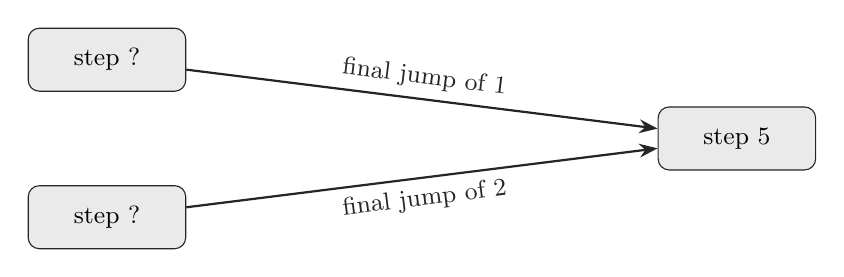
\begin{tikzpicture}[>=Stealth,every node/.style={font=\small},box/.style={draw=teal,rounded corners,minimum width=20mm,minimum height=8mm,fill=wash},arr/.style={->,thick,teal}]\node[box] (a) at (0,1) {step ?};\node[box] (b) at (0,-1) {step ?};\node[box] (c) at (8,0) {step 5};\draw[arr] (a)--node[above,sloped]{final jump of 1}(c);\draw[arr] (b)--node[below,sloped]{final jump of 2}(c);\end{tikzpicture}\end{center}
\par\medskip\textbf{Worked answer.} The last move starts at step 4 with a jump of 1, or at step 3 with a jump of 2. Extend each earlier route once. The groups cannot overlap because their last moves differ: 5 + 3 = 8.

\textbf{Diagram for the answer.}\par\begin{center}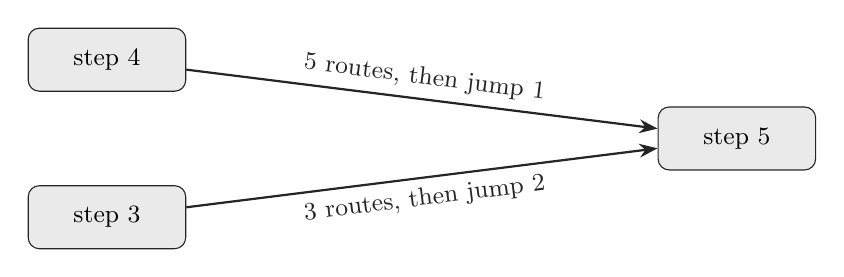
\begin{tikzpicture}[>=Stealth,every node/.style={font=\small},box/.style={draw=teal,rounded corners,minimum width=20mm,minimum height=8mm,fill=wash},arr/.style={->,thick,teal}]\node[box] (a) at (0,1) {step 4};\node[box] (b) at (0,-1) {step 3};\node[box] (c) at (8,0) {step 5};\draw[arr] (a)--node[above,sloped]{5 routes, then jump 1}(c);\draw[arr] (b)--node[below,sloped]{3 routes, then jump 2}(c);\end{tikzpicture}\end{center}
Each route to step 5 has exactly one last move. Removing that move leaves a route to step 4 or step 3. These two groups include every route, and no route is in both groups, so adding the counts neither misses nor repeats a route.

\end{qblock}
\end{qblock}\par\medskip{\color{lightink}\hrule height .4pt}\bigskip
\par\markboth{Where recursion stops}{}\begin{qblock}\begin{qblock}[0.95]
\qtopic{L1-07}{Where recursion stops}
{\small\color{quiet}Staircase: count, remember, then loop}\par\medskip
\textbf{Question.} Let ways(n) return the number of routes from the ground to target step n, using jumps of 1 or 2. What should ways(0) and ways(-1) return? Use these answers to work out ways(1).

\par\medskip\textbf{Worked answer.} ways(0) = 1: the empty list is one way to climb zero steps. ways(-1) = 0: positive jumps cannot finish below the ground. Therefore ways(1) = ways(0) + ways(-1) = 1.

\end{qblock}
\end{qblock}\par\medskip{\color{lightink}\hrule height .4pt}\bigskip
\par\markboth{The slow recursive program}{}\begin{qblock}\begin{qblock}[0.95]
\qtopic{L1-08}{The slow recursive program}
{\small\color{quiet}Staircase: count, remember, then loop}\par\medskip
\textbf{Question.} Write stairs\_slow(n), the number of staircase routes to step n with jumps of 1 or 2. Start with the stopping cases, then ask about the two possible starting steps of the final jump. Draw every call made for stairs\_slow(3) and write the returned count beside it.

\par\smallskip{\small\textbf{Start with:}}\par\smallskip\noindent\colorbox{codepaper}{\parbox{\dimexpr\linewidth-2\fboxsep\relax}{\small\ttfamily\raggedright def stairs\_slow(n):\\\hspace*{2.4em}return None  \# Replace with your answer.}}\par
{\small\textbf{What each function returns.}\par stairs\_slow(n): the number of ordered routes to step n using jumps of 1 or 2.\par }
{\small\textbf{Hints.}}\begin{itemize}\item Which targets can you answer without a smaller call? Think about 0 and about negative targets.\item The last move is 1 or 2 steps. Which smaller targets do those leave?\end{itemize}
\par\medskip\textbf{Worked answer.} stairs\_slow(3) returns 3. It calls stairs\_slow(2) and stairs\_slow(1); stairs\_slow(2) calls stairs\_slow(1) and stairs\_slow(0). Each stairs\_slow(1) calls stairs\_slow(0) and stairs\_slow(-1). Return 1 at target 0 and 0 at target -1. Then stairs\_slow(1) returns 1, stairs\_slow(2) returns 2, and stairs\_slow(3) returns 2 + 1 = 3.

Each line of the trace shows one call and its returned count. Indentation identifies the calls it makes. Repeated lines are separate calls, not reused answers.

\textbf{Complete call trace.} Each arrow gives the returned count.
\begin{lstlisting}[language={}]
stairs_slow(3) -> 3
|-- stairs_slow(2) -> 2
|   |-- stairs_slow(1) -> 1
|   |   `-- stairs_slow(0) -> 1
|   `-- stairs_slow(0) -> 1
`-- stairs_slow(1) -> 1
    `-- stairs_slow(0) -> 1
\end{lstlisting}
\end{qblock}
\begin{qblock}[0.95]
\medskip\textbf{One complete Python implementation: stairs\_slow.}\label{ans-stairs_slow}\par
\begin{lstlisting}[style=numbered]
def stairs_slow(n):
    if n < 0:
        return 0
    if n == 0:
        return 1
    return stairs_slow(n - 1) + stairs_slow(n - 2)
\end{lstlisting}
\textbf{Check.} Run this after the function above.
\begin{lstlisting}
print(stairs_slow(5))
\end{lstlisting}
\textbf{Expected output.}
\begin{lstlisting}[language={}]
8
\end{lstlisting}
\textbf{Recursion depth.} Python stops recursion at about 1,000 nested calls by default, so this recursive version is for small inputs and the small and edge test files only. Use the iterative version for the medium and large files.

\end{qblock}
\end{qblock}\par\medskip{\color{lightink}\hrule height .4pt}\bigskip
\par\markboth{Repeated questions in the call tree}{}\begin{qblock}\begin{qblock}[0.95]
\qtopic{L1-09}{Repeated questions in the call tree}
{\small\color{quiet}Staircase: count, remember, then loop}\par\medskip
\textbf{Question.} The diagram shows the first three levels of calls made while counting routes to step 5. Circle calls with the same input. What work does the second call to ways(3) repeat?

\textbf{Diagram supplied with the question.}\par\begin{center}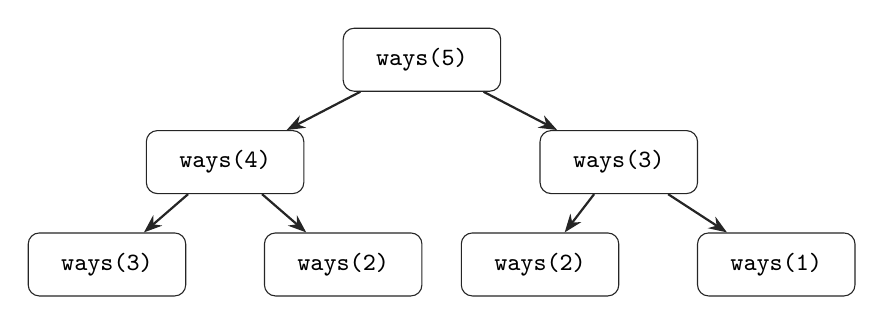
\begin{tikzpicture}[>=Stealth,every node/.style={font=\small},box/.style={draw=teal,rounded corners,minimum width=20mm,minimum height=8mm,fill=wash},arr/.style={->,thick,teal}]\node[box,fill=paper] (a) at (5,0) {\texttt{ways(5)}};\node[box,fill=paper] (b) at (2.5,-1.3) {\texttt{ways(4)}};\node[box,fill=paper] (c) at (7.5,-1.3) {\texttt{ways(3)}};\node[box,fill=paper] (d) at (1,-2.6) {\texttt{ways(3)}};\node[box,fill=paper] (e) at (4,-2.6) {\texttt{ways(2)}};\node[box,fill=paper] (f) at (6.5,-2.6) {\texttt{ways(2)}};\node[box,fill=paper] (g) at (9.5,-2.6) {\texttt{ways(1)}};\draw[arr] (a)--(b);\draw[arr] (a)--(c);\draw[arr] (b)--(d);\draw[arr] (b)--(e);\draw[arr] (c)--(f);\draw[arr] (c)--(g);\end{tikzpicture}\end{center}
\par\medskip\textbf{Worked answer.} The displayed levels contain two calls to ways(3) and two to ways(2). Each call to ways(3) asks for the same route count, but both rebuild its smaller calls. The drawing stops early: each displayed call with a positive input would continue branching until a stopping case.

\textbf{Diagram for the answer.}\par\begin{center}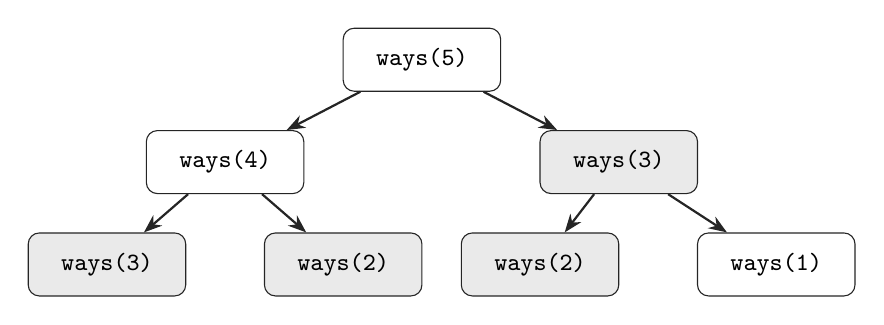
\begin{tikzpicture}[>=Stealth,every node/.style={font=\small},box/.style={draw=teal,rounded corners,minimum width=20mm,minimum height=8mm,fill=wash},arr/.style={->,thick,teal}]\node[box,fill=paper] (a) at (5,0) {\texttt{ways(5)}};\node[box,fill=paper] (b) at (2.5,-1.3) {\texttt{ways(4)}};\node[box,fill=wash] (c) at (7.5,-1.3) {\texttt{ways(3)}};\node[box,fill=wash] (d) at (1,-2.6) {\texttt{ways(3)}};\node[box,fill=wash] (e) at (4,-2.6) {\texttt{ways(2)}};\node[box,fill=wash] (f) at (6.5,-2.6) {\texttt{ways(2)}};\node[box,fill=paper] (g) at (9.5,-2.6) {\texttt{ways(1)}};\draw[arr] (a)--(b);\draw[arr] (a)--(c);\draw[arr] (b)--(d);\draw[arr] (b)--(e);\draw[arr] (c)--(f);\draw[arr] (c)--(g);\end{tikzpicture}\end{center}
The two displayed ways(3) calls both calculate ways(2) and ways(1), and those calls branch again. The two ways(2) calls also repeat work. A saved answer lets a later call with the same input return immediately.

\end{qblock}
\end{qblock}\par\medskip{\color{lightink}\hrule height .4pt}\bigskip
\par\markboth{A cache keeps an answer}{}\begin{qblock}\begin{qblock}[0.95]
\qtopic{L1-10}{A cache keeps an answer}
{\small\color{quiet}Staircase: count, remember, then loop}\par\medskip
\textbf{Question.} A cache is a dictionary that saves an answer under the input that produced it. We have found 5 routes to step 4. Complete cache[?] = ?. What should a later call to ways(4) return, and which work can it skip?

\par\medskip\textbf{Worked answer.} Store cache[4] = 5. Key 4 identifies the step. Value 5 is its route count. A later call reads 5 immediately instead of exploring ways(3) and ways(2) again.

\end{qblock}
\begin{qblock}[0.95]
\medskip\textbf{One complete Python implementation: stairs\_cached.}\label{ans-stairs_cached}\par
\begin{lstlisting}[style=numbered]
def stairs_cached(n):
    cache = {0: 1}
    def ways(step):
        if step < 0:
            return 0
        if step not in cache:
            cache[step] = ways(step - 1) + ways(step - 2)
        return cache[step]
    return ways(n)
\end{lstlisting}
\textbf{Check.} Run this after the function above.
\begin{lstlisting}
print(stairs_cached(20))
\end{lstlisting}
\textbf{Expected output.}
\begin{lstlisting}[language={}]
10946
\end{lstlisting}
\textbf{Recursion depth.} Python stops recursion at about 1,000 nested calls by default, so this recursive version is for small inputs and the small and edge test files only. Use the iterative version for the medium and large files.

\end{qblock}
\end{qblock}\par\medskip{\color{lightink}\hrule height .4pt}\bigskip
\par\markboth{Fast work can still mean deep recursion}{}\begin{qblock}\begin{qblock}[0.95]
\qtopic{L1-11}{Fast work can still mean deep recursion}
{\small\color{quiet}Staircase: count, remember, then loop}\par\medskip
\textbf{Question.} Caching removes repeated work. Why can a large staircase input still cause RecursionError in Python? What does iteration change?

\par\medskip\textbf{Worked answer.} The calls for n, n - 1, n - 2 and so on can remain active together. Caching does not shorten that chain. Python limits nested calls. A loop fills answers without building this recursive call chain.

For example, the first call for target n can wait for n - 1, which waits for n - 2. Those calls remain on the stack together. A cache reduces how often an answer is computed; a loop also removes this chain of waiting calls.

\end{qblock}
\begin{qblock}[0.95]
\medskip\textbf{One complete Python implementation: recursion\_demo.}\label{ans-recursion_demo}\par
\begin{lstlisting}[style=numbered]
import sys

def recursion_demo():
    def descend(n):
        if n == 0:
            return 0
        return 1 + descend(n - 1)
    try:
        descend(sys.getrecursionlimit() + 10)
    except RecursionError:
        return 'Caught RecursionError: too many nested calls.'
    return 'No RecursionError: the limit was not reached.'
\end{lstlisting}
\textbf{Check.} Run this after the function above.
\begin{lstlisting}
print(recursion_demo())
\end{lstlisting}
\textbf{Expected output.}
\begin{lstlisting}[language={}]
Caught RecursionError: too many nested calls.
\end{lstlisting}
\end{qblock}
\end{qblock}\par\medskip{\color{lightink}\hrule height .4pt}\bigskip
\par\markboth{Build the table in order}{}\begin{qblock}\begin{qblock}[0.95]
\qtopic{L1-12}{Build the table in order}
{\small\color{quiet}Staircase: count, remember, then loop}\par\medskip
\textbf{Question.} Write stairs\_table(n) using a loop. First fill ways[step], the route count, for steps 0 through 5. Which earlier count is available at step 1? Which two are needed from step 2 onwards? Use that order in your code.

\par\smallskip{\small\textbf{Start with:}}\par\smallskip\noindent\colorbox{codepaper}{\parbox{\dimexpr\linewidth-2\fboxsep\relax}{\small\ttfamily\raggedright def stairs\_table(n):\\\hspace*{2.4em}return None  \# Replace with your answer.}}\par
{\small\textbf{What each function returns.}\par stairs\_table(n): the number of ordered routes to step n using jumps of 1 or 2.\par }
{\small\textbf{Hints.}}\begin{itemize}\item How long must the list be so that ways[n] exists?\item Which entry do you know before the loop starts?\item When you fill ways[step], which entries must already be filled?\end{itemize}
\textbf{Table supplied with the question.}\par\par\medskip \begingroup\small\setlength{\tabcolsep}{4pt}\renewcommand{\arraystretch}{1.35}\begin{tabularx}{\linewidth}{>{\raggedright\arraybackslash}l>{\raggedright\arraybackslash}X>{\raggedright\arraybackslash}X>{\raggedright\arraybackslash}X>{\raggedright\arraybackslash}X>{\raggedright\arraybackslash}X>{\raggedright\arraybackslash}X}\toprule\textbf{Step} & \textbf{0} & \textbf{1} & \textbf{2} & \textbf{3} & \textbf{4} & \textbf{5}\\\midrule
ways[step] & 1 & ? & ? & ? & ? & ?\\
\bottomrule\end{tabularx}\endgroup\par\medskip 
\par\medskip\textbf{Worked answer.} The counts are [1, 1, 2, 3, 5, 8]. Step 1 reads only ways[0]. Each step s from 2 onwards reads ways[s - 1] and ways[s - 2]. For step 5, those counts are 5 and 3, giving 8. Increasing step order ensures both earlier answers exist.

\textbf{Completed table.}\par\par\medskip \begingroup\small\setlength{\tabcolsep}{4pt}\renewcommand{\arraystretch}{1.35}\begin{tabularx}{\linewidth}{>{\raggedright\arraybackslash}l>{\raggedright\arraybackslash}X>{\raggedright\arraybackslash}X>{\raggedright\arraybackslash}X>{\raggedright\arraybackslash}X>{\raggedright\arraybackslash}X>{\raggedright\arraybackslash}X}\toprule\textbf{Step} & \textbf{0} & \textbf{1} & \textbf{2} & \textbf{3} & \textbf{4} & \textbf{5}\\\midrule
ways[step] & 1 & 1 & 2 & 3 & 5 & 8\\
\bottomrule\end{tabularx}\endgroup\par\medskip 
The index is a step number; the stored value counts routes. Start with one empty route at step 0. At step 1 there is no predecessor step -1 in the table, so read only step 0. From step 2 onwards, both predecessors exist.

\end{qblock}
\begin{qblock}[0.95]
\medskip\textbf{One complete Python implementation: stairs\_table.}\label{ans-stairs_table}\par
\begin{lstlisting}[style=numbered]
def stairs_table(n):
    ways = [0] * (n + 1)
    ways[0] = 1
    for step in range(1, n + 1):
        ways[step] = ways[step - 1]
        if step >= 2:
            ways[step] += ways[step - 2]
    return ways[n]
\end{lstlisting}
\textbf{Check.} Run this after the function above.
\begin{lstlisting}
print([stairs_table(n) for n in range(6)])
\end{lstlisting}
\textbf{Expected output.}
\begin{lstlisting}[language={}]
[1, 1, 2, 3, 5, 8]
\end{lstlisting}
\end{qblock}
\end{qblock}\par\medskip{\color{lightink}\hrule height .4pt}\bigskip
\par\markboth{Your turn: jumps of 1 or 3}{}\begin{qblock}\begin{qblock}[0.95]
\qtopic{L1-13}{Your turn: jumps of 1 or 3}
{\small\color{quiet}Staircase: count, remember, then loop}\par\medskip
\textbf{Question.} Write stairs\_13(n) by adapting stairs\_table from L1-12. Allow only jumps of 1 or 3, never 2. First fill the counts for steps 0 through 7, then write and test your code.

\par\smallskip{\small\textbf{Start with:}}\par\smallskip\noindent\colorbox{codepaper}{\parbox{\dimexpr\linewidth-2\fboxsep\relax}{\small\ttfamily\raggedright def stairs\_13(n):\\\hspace*{2.4em}return None  \# Replace with your answer.}}\par
{\small\textbf{What each function returns.}\par stairs\_13(n): the number of ordered routes to step n using jumps of 1 or 3.\par }
{\small\textbf{Hints.}}\begin{itemize}\item Which line of stairs\_table depends on the allowed jumps?\item A jump can only start from a step that exists. What must be true before you read an earlier entry?\end{itemize}
\textbf{Table supplied with the question.}\par\par\medskip \begingroup\small\setlength{\tabcolsep}{4pt}\renewcommand{\arraystretch}{1.35}\begin{tabularx}{\linewidth}{>{\raggedright\arraybackslash}l>{\raggedright\arraybackslash}X>{\raggedright\arraybackslash}X>{\raggedright\arraybackslash}X>{\raggedright\arraybackslash}X>{\raggedright\arraybackslash}X>{\raggedright\arraybackslash}X>{\raggedright\arraybackslash}X>{\raggedright\arraybackslash}X}\toprule\textbf{Step} & \textbf{0} & \textbf{1} & \textbf{2} & \textbf{3} & \textbf{4} & \textbf{5} & \textbf{6} & \textbf{7}\\\midrule
ways[step] & 1 &  &  &  &  &  &  & \\
\bottomrule\end{tabularx}\endgroup\par\medskip 
\par\medskip\textbf{Worked answer.} The counts are [1, 1, 1, 2, 3, 4, 6, 9]. For step 7, the last jump begins at step 6 or step 4, giving 6 + 3 = 9. Use jumps (1, 3) and ignore negative predecessor steps.

\textbf{Completed table.}\par\par\medskip \begingroup\small\setlength{\tabcolsep}{4pt}\renewcommand{\arraystretch}{1.35}\begin{tabularx}{\linewidth}{>{\raggedright\arraybackslash}l>{\raggedright\arraybackslash}X>{\raggedright\arraybackslash}X>{\raggedright\arraybackslash}X>{\raggedright\arraybackslash}X>{\raggedright\arraybackslash}X>{\raggedright\arraybackslash}X>{\raggedright\arraybackslash}X>{\raggedright\arraybackslash}X}\toprule\textbf{Step} & \textbf{0} & \textbf{1} & \textbf{2} & \textbf{3} & \textbf{4} & \textbf{5} & \textbf{6} & \textbf{7}\\\midrule
ways[step] & 1 & 1 & 1 & 2 & 3 & 4 & 6 & 9\\
\bottomrule\end{tabularx}\endgroup\par\medskip 
\end{qblock}
\begin{qblock}[0.95]
\medskip\textbf{One complete Python implementation: stairs\_13.}\label{ans-stairs_13}\par
\begin{lstlisting}[style=numbered]
def stairs_13(n):
    ways = [0] * (n + 1)
    ways[0] = 1
    for step in range(1, n + 1):
        for jump in (1, 3):
            if step >= jump:
                ways[step] += ways[step - jump]
    return ways[n]
\end{lstlisting}
\textbf{Check.} Run this after the function above.
\begin{lstlisting}
print([stairs_13(n) for n in range(8)])
\end{lstlisting}
\textbf{Expected output.}
\begin{lstlisting}[language={}]
[1, 1, 1, 2, 3, 4, 6, 9]
\end{lstlisting}
\end{qblock}
\end{qblock}\par\medskip{\color{lightink}\hrule height .4pt}\bigskip
\par\markboth{Frog: cost belongs to a whole route}{}\begin{qblock}\begin{qblock}[0.95]
\qtopic{L1-14}{Frog: cost belongs to a whole route}
{\small\color{quiet}Frog: compare complete route costs}\par\medskip
\textbf{Question.} Number the stones 0, 1 and 2; their heights are [10, 20, 30]. A frog starts at stone 0 and may jump forward one or two positions. A jump costs the absolute height difference, so a drop of 10 also costs 10. List all routes to stone 2 and add the jump costs for each.

\par\medskip\textbf{Worked answer.} The routes are 0, 1, 2 with cost 10 + 10 = 20, and 0, 2 with cost 20. Both are optimal. A cost is never negative: abs(10 - 30) = 20.

\end{qblock}
\end{qblock}\par\medskip{\color{lightink}\hrule height .4pt}\bigskip
\par\markboth{A greedy choice can fail}{}\begin{qblock}\begin{qblock}[0.95]
\qtopic{L1-15}{A greedy choice can fail}
{\small\color{quiet}Frog: compare complete route costs}\par\medskip
\textbf{Question.} Use heights [20, 50, 30, 40, 10, 10], at stones 0 through 5. At each stone, choose the cheaper of the next two legal jumps; if costs tie, choose the farther stone. Trace this greedy route and its total cost. Can another complete route cost less?

\textbf{Table supplied with the question.}\par\par\medskip \begingroup\small\setlength{\tabcolsep}{4pt}\renewcommand{\arraystretch}{1.35}\begin{tabularx}{\linewidth}{>{\raggedright\arraybackslash}l>{\raggedright\arraybackslash}X>{\raggedright\arraybackslash}X>{\raggedright\arraybackslash}X>{\raggedright\arraybackslash}X>{\raggedright\arraybackslash}X>{\raggedright\arraybackslash}X}\toprule\textbf{Stone i} & \textbf{0} & \textbf{1} & \textbf{2} & \textbf{3} & \textbf{4} & \textbf{5}\\\midrule
heights[i] & 20 & 50 & 30 & 40 & 10 & 10\\
\bottomrule\end{tabularx}\endgroup\par\medskip 
\par\medskip\textbf{Worked answer.} Greedy can take stones 0, 2, 3, 5: cost 10 + 10 + 30 = 50. The optimal route 0, 2, 4, 5 costs 10 + 20 + 0 = 30. Paying more at stone 2 saves cost later.

\textbf{Completed table.}\par\par\medskip \begingroup\small\setlength{\tabcolsep}{4pt}\renewcommand{\arraystretch}{1.35}\begin{tabularx}{\linewidth}{>{\raggedright\arraybackslash}l>{\raggedright\arraybackslash}X>{\raggedright\arraybackslash}X>{\raggedright\arraybackslash}X>{\raggedright\arraybackslash}X>{\raggedright\arraybackslash}X>{\raggedright\arraybackslash}X>{\raggedright\arraybackslash}X}\toprule\textbf{Jump into stone i} & \textbf{0} & \textbf{1} & \textbf{2} & \textbf{3} & \textbf{4} & \textbf{5} & \textbf{Total}\\\midrule
heights[i] & 20 & 50 & 30 & 40 & 10 & 10 & \\
greedy 0, 2, 3, 5 & start &  & 10 & 10 &  & 30 & 50\\
best 0, 2, 4, 5 & start &  & 10 &  & 20 & 0 & 30\\
\bottomrule\end{tabularx}\endgroup\par\medskip 
At stone 2, greedy pays 10 to reach stone 3 instead of 20 to reach stone 4. However, it then pays 30 to reach height 10. The alternative pays 20 now and 0 on the final jump: 10 + 20 + 0 = 30.

\end{qblock}
\end{qblock}\par\medskip{\color{lightink}\hrule height .4pt}\bigskip
\par\markboth{Frog: ask about the last jump}{}\begin{qblock}\begin{qblock}[0.95]
\qtopic{L1-16}{Frog: ask about the last jump}
{\small\color{quiet}Frog: compare complete route costs}\par\medskip
\textbf{Question.} Write frog\_slow(heights) with recursive helper cost(i): the cheapest total cost from stone 0 to stone i. Which earlier stones can supply the last jump? Explore both possibilities.

\par\smallskip{\small\textbf{Start with:}}\par\smallskip\noindent\colorbox{codepaper}{\parbox{\dimexpr\linewidth-2\fboxsep\relax}{\small\ttfamily\raggedright def frog\_slow(heights):\\\hspace*{2.4em}def cost(i):\\\hspace*{4.8em}return None  \# Your helper goes here.\\\hspace*{2.4em}return cost(len(heights) - 1)}}\par
{\small\textbf{What each function returns.}\par frog\_slow(heights): the cheapest total cost from stone 0 to the last stone.\par cost(i): the cheapest total cost from stone 0 to stone i, including all jumps along the route.\par }
{\small\textbf{Hints.}}\begin{itemize}\item What is the smallest i you can answer directly?\item Which earlier stones can the last jump into stone i start from?\item What does cost(i) need to know about each of those stones?\end{itemize}
\par\medskip\textbf{Worked answer.} Try i - 1 and, when it exists, i - 2. Add the last jump cost to the cheapest cost of reaching that earlier stone, then take the minimum. cost(0) is 0 because the frog starts there.

For stone 2 in the six-stone example, the route through stone 1 costs 30 + abs(30 - 50) = 50. The direct jump from stone 0 costs 0 + abs(30 - 20) = 10. The minimum is 10. Both candidates include the complete earlier route cost.

\end{qblock}
\begin{qblock}[0.95]
\medskip\textbf{One complete Python implementation: frog\_slow.}\label{ans-frog_slow}\par
\begin{lstlisting}[style=numbered]
def frog_slow(heights):
    def cost(i):
        if i == 0:
            return 0
        one = cost(i - 1) + abs(heights[i] - heights[i - 1])
        if i == 1:
            return one
        two = cost(i - 2) + abs(heights[i] - heights[i - 2])
        return min(one, two)
    return cost(len(heights) - 1)
\end{lstlisting}
\textbf{Check.} Run this after the function above.
\begin{lstlisting}
print(frog_slow([20, 50, 30, 40, 10, 10]))
\end{lstlisting}
\textbf{Expected output.}
\begin{lstlisting}[language={}]
30
\end{lstlisting}
\textbf{Recursion depth.} Python stops recursion at about 1,000 nested calls by default, so this recursive version is for small inputs and the small and edge test files only. Use the iterative version for the medium and large files.

\end{qblock}
\end{qblock}\par\medskip{\color{lightink}\hrule height .4pt}\bigskip
\par\markboth{Frog: cache the stone number}{}\begin{qblock}\begin{qblock}[0.95]
\qtopic{L1-17}{Frog: cache the stone number}
{\small\color{quiet}Frog: compare complete route costs}\par\medskip
\textbf{Question.} In the recursive Frog solution, what is the cache key? Why can different routes that reach the same stone share an answer?

\par\medskip\textbf{Worked answer.} The key is the stone index i. cost(i) always asks for the cheapest cost from the fixed start to that stone. The fixed height list and allowed jumps are the same in every call, so one answer per i is enough.

\end{qblock}
\begin{qblock}[0.95]
\medskip\textbf{One complete Python implementation: frog\_cached.}\label{ans-frog_cached}\par
\begin{lstlisting}[style=numbered]
def frog_cached(heights):
    cache = {0: 0}
    def cost(i):
        if i not in cache:
            one = cost(i - 1) + abs(heights[i] - heights[i - 1])
            answer = one
            if i >= 2:
                two = cost(i - 2) + abs(heights[i] - heights[i - 2])
                answer = min(one, two)
            cache[i] = answer
        return cache[i]
    return cost(len(heights) - 1)
\end{lstlisting}
\textbf{Check.} Run this after the function above.
\begin{lstlisting}
print(frog_cached([20, 50, 30, 40, 10, 10]))
\end{lstlisting}
\textbf{Expected output.}
\begin{lstlisting}[language={}]
30
\end{lstlisting}
\textbf{Recursion depth.} Python stops recursion at about 1,000 nested calls by default, so this recursive version is for small inputs and the small and edge test files only. Use the iterative version for the medium and large files.

\end{qblock}
\end{qblock}\par\medskip{\color{lightink}\hrule height .4pt}\bigskip
\par\markboth{Frog: write the iterative solution}{}\begin{qblock}\begin{qblock}[0.95]
\qtopic{L1-18}{Frog: write the iterative solution}
{\small\color{quiet}Frog: compare complete route costs}\par\medskip
\textbf{Question.} Write frog\_table(heights) using a loop. Return the cheapest total cost from stone 0 to the last stone. First fill best[i] for heights [20, 50, 30, 40, 10, 10], then turn those steps into Python code. Explain why the loop runs from left to right. Test your function on these heights.

\par\smallskip{\small\textbf{Start with:}}\par\smallskip\noindent\colorbox{codepaper}{\parbox{\dimexpr\linewidth-2\fboxsep\relax}{\small\ttfamily\raggedright def frog\_table(heights):\\\hspace*{2.4em}return None  \# Replace with your answer.}}\par
{\small\textbf{What each function returns.}\par frog\_table(heights): the cheapest total cost from stone 0 to the last stone.\par }
{\small\textbf{Hints.}}\begin{itemize}\item What is best[0], before any jump?\item Which earlier entries does best[i] need, and are they filled when the loop reaches i?\end{itemize}
\textbf{Table supplied with the question.}\par\par\medskip \begingroup\small\setlength{\tabcolsep}{4pt}\renewcommand{\arraystretch}{1.35}\begin{tabularx}{\linewidth}{>{\raggedright\arraybackslash}l>{\raggedright\arraybackslash}X>{\raggedright\arraybackslash}X>{\raggedright\arraybackslash}X>{\raggedright\arraybackslash}X>{\raggedright\arraybackslash}X>{\raggedright\arraybackslash}X}\toprule\textbf{Stone i} & \textbf{0} & \textbf{1} & \textbf{2} & \textbf{3} & \textbf{4} & \textbf{5}\\\midrule
heights[i] & 20 & 50 & 30 & 40 & 10 & 10\\
best[i] & 0 & ? & ? & ? & ? & ?\\
\bottomrule\end{tabularx}\endgroup\par\medskip 
\par\medskip\textbf{Worked answer.} The costs are [0, 30, 10, 20, 30, 30]. For stone 4, the two totals are 20 + 30 = 50 and 10 + 20 = 30. Every dependency has a smaller index, so it is already computed.

\textbf{Completed table.}\par\par\medskip \begingroup\small\setlength{\tabcolsep}{4pt}\renewcommand{\arraystretch}{1.35}\begin{tabularx}{\linewidth}{>{\raggedright\arraybackslash}l>{\raggedright\arraybackslash}X>{\raggedright\arraybackslash}X>{\raggedright\arraybackslash}X>{\raggedright\arraybackslash}X>{\raggedright\arraybackslash}X>{\raggedright\arraybackslash}X}\toprule\textbf{Stone i} & \textbf{0} & \textbf{1} & \textbf{2} & \textbf{3} & \textbf{4} & \textbf{5}\\\midrule
heights[i] & 20 & 50 & 30 & 40 & 10 & 10\\
best[i] & 0 & 30 & 10 & 20 & 30 & 30\\
\bottomrule\end{tabularx}\endgroup\par\medskip 
For the last stone, coming from stone 4 costs 30 + abs(10 - 10) = 30. Coming from stone 3 costs 20 + abs(10 - 40) = 50. Store 30. Do not add every entry in best: each entry already measures a complete route from stone 0.

\end{qblock}
\begin{qblock}[0.95]
\medskip\textbf{One complete Python implementation: frog\_table.}\label{ans-frog_table}\par
\begin{lstlisting}[style=numbered]
def frog_table(heights):
    best = [0] * len(heights)
    for i in range(1, len(heights)):
        best[i] = best[i - 1] + abs(heights[i] - heights[i - 1])
        if i >= 2:
            two = best[i - 2] + abs(heights[i] - heights[i - 2])
            best[i] = min(best[i], two)
    return best[-1]
\end{lstlisting}
\textbf{Check.} Run this after the function above.
\begin{lstlisting}
print(frog_table([20, 50, 30, 40, 10, 10]))
\end{lstlisting}
\textbf{Expected output.}
\begin{lstlisting}[language={}]
30
\end{lstlisting}
\end{qblock}
\end{qblock}\par\medskip{\color{lightink}\hrule height .4pt}\bigskip
\par\markboth{Your turn: a new Frog instance}{}\begin{qblock}\begin{qblock}[0.95]
\qtopic{L1-19}{Your turn: a new Frog instance}
{\small\color{quiet}Frog: compare complete route costs}\par\medskip
\textbf{Question.} Test your frog\_table(heights) from L1-18. For heights [10, 30, 20, 40], first predict best[i] and give one cheapest route, then run your function. Next predict and test the answer for 100,000 equal-height stones. Explain why uncached recursion is unsuitable for that large test.

\textbf{Table supplied with the question.}\par\par\medskip \begingroup\small\setlength{\tabcolsep}{4pt}\renewcommand{\arraystretch}{1.35}\begin{tabularx}{\linewidth}{>{\raggedright\arraybackslash}X>{\raggedright\arraybackslash}X>{\raggedright\arraybackslash}X>{\raggedright\arraybackslash}X>{\raggedright\arraybackslash}X}\toprule\textbf{Stone i} & \textbf{0} & \textbf{1} & \textbf{2} & \textbf{3}\\\midrule
heights[i] & 10 & 30 & 20 & 40\\
best[i] & 0 &  &  & \\
\bottomrule\end{tabularx}\endgroup\par\medskip 
\par\medskip\textbf{Worked answer.} The costs are [0, 20, 10, 30]; route 0, 2, 3 costs 30. With 100,000 equal heights the answer is 0 because every jump costs 0. Iteration fills one cost per stone. Uncached recursion repeatedly explores the same earlier stones and also builds a deep call stack.

\textbf{Completed table.}\par\par\medskip \begingroup\small\setlength{\tabcolsep}{4pt}\renewcommand{\arraystretch}{1.35}\begin{tabularx}{\linewidth}{>{\raggedright\arraybackslash}X>{\raggedright\arraybackslash}X>{\raggedright\arraybackslash}X>{\raggedright\arraybackslash}X>{\raggedright\arraybackslash}X}\toprule\textbf{Stone i} & \textbf{0} & \textbf{1} & \textbf{2} & \textbf{3}\\\midrule
heights[i] & 10 & 30 & 20 & 40\\
best[i] & 0 & 20 & 10 & 30\\
\bottomrule\end{tabularx}\endgroup\par\medskip 
For stone 3, coming from stone 2 costs 10 + abs(40 - 20) = 30. Coming from stone 1 costs 20 + abs(40 - 30) = 30 as well. Thus 0, 1, 3 is another cheapest route. The large test below uses iteration only.

\end{qblock}
\begin{qblock}[0.95]
\medskip\textbf{Same implementation as L1-18} (\texttt{frog\_table}, page~\pageref{ans-frog_table}).\par\textbf{Check.} Run this after that function.
\begin{lstlisting}
print(frog_table([10, 30, 20, 40]))
print(frog_table([7] * 100000))
\end{lstlisting}
\textbf{Expected output.}
\begin{lstlisting}[language={}]
30
0
\end{lstlisting}
\end{qblock}
\end{qblock}\par\medskip{\color{lightink}\hrule height .4pt}\bigskip
\par\markboth{Counting and minimising}{}\begin{qblock}\begin{qblock}[0.95]
\qtopic{L1-20}{Counting and minimising}
{\small\color{quiet}Frog: compare complete route costs}\par\medskip
\textbf{Question.} Both staircase and Frog inspect earlier states. Why does staircase add their answers, while Frog takes a minimum? What does each table entry mean?

\par\medskip\textbf{Worked answer.} Staircase counts all routes, so disjoint last-move groups contribute by addition. Frog asks for one cheapest cost, so competing last-jump totals combine with min. State meanings determine the operation.

ways[step] counts routes to that step. best[i] is the cheapest complete cost to stone i. Staircase includes both last-move groups; Frog chooses the cheaper of the two last-jump totals.

\end{qblock}
\end{qblock}\par\medskip{\color{lightink}\hrule height .4pt}\bigskip
\par\markboth{Frog: recover a cheapest path}{}\begin{qblock}\begin{qblock}[0.95]
\qtopic{L1-21 / OPTIONAL EXTENSION}{Frog: recover a cheapest path}
{\small\color{quiet}Extension: recover a cheapest Frog route}\par\medskip
\textbf{Question.} Extend your cost solution: write frog\_path(heights), returning (cost, path), where path lists stone indices from start to finish. For heights [20, 50, 30, 40, 10, 10], record in previous[i] which earlier stone gives best[i]. Use -1 for the start. On equal costs keep i - 1. Trace backwards from the last stone, then return the path in forward order.

\par\smallskip{\small\textbf{Start with:}}\par\smallskip\noindent\colorbox{codepaper}{\parbox{\dimexpr\linewidth-2\fboxsep\relax}{\small\ttfamily\raggedright def frog\_path(heights):\\\hspace*{2.4em}return None  \# Replace with your answer.}}\par
{\small\textbf{What each function returns.}\par frog\_path(heights): a pair (cost, path): the minimum total cost and a list of stone indices from 0 to the last stone. On equal candidate costs, keep the predecessor i - 1.\par }
{\small\textbf{Hints.}}\begin{itemize}\item When a candidate becomes the cheapest, what earlier stone should you remember?\item Start at the last stone and follow the saved indices. How will you recognise the start?\item In which order did you collect the stones, and which order should you return?\end{itemize}
\par\medskip\textbf{Worked answer.} The previous list is [-1, 0, 0, 2, 2, 4]. Starting at stone 5, follow 5, 4, 2, 0, then stop at -1. Reverse the collected list to get [0, 2, 4, 5]. The function returns (30, [0, 2, 4, 5]): the jump costs are 10 + 20 + 0 = 30.

\textbf{Completed table.}\par\par\medskip \begingroup\small\setlength{\tabcolsep}{4pt}\renewcommand{\arraystretch}{1.35}\begin{tabularx}{\linewidth}{>{\raggedright\arraybackslash}l>{\raggedright\arraybackslash}X>{\raggedright\arraybackslash}X>{\raggedright\arraybackslash}X>{\raggedright\arraybackslash}X>{\raggedright\arraybackslash}X>{\raggedright\arraybackslash}X}\toprule\textbf{Stone i} & \textbf{0} & \textbf{1} & \textbf{2} & \textbf{3} & \textbf{4} & \textbf{5}\\\midrule
heights[i] & 20 & 50 & 30 & 40 & 10 & 10\\
best[i] & 0 & 30 & 10 & 20 & 30 & 30\\
previous[i] & -1 & 0 & 0 & 2 & 2 & 4\\
\bottomrule\end{tabularx}\endgroup\par\medskip 
\par\smallskip\resizebox{\linewidth}{!}{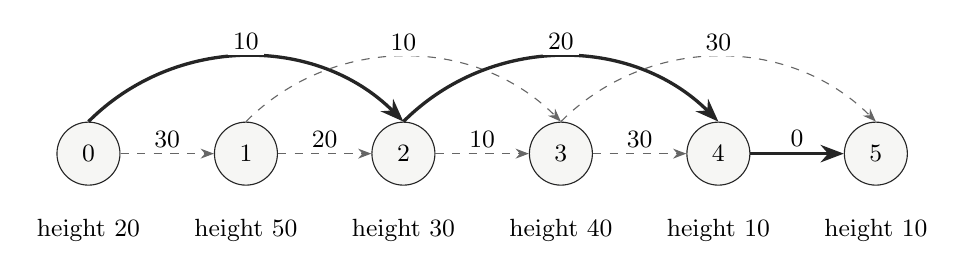
\begin{tikzpicture}[x=1cm,y=1cm,>=Stealth,every node/.style={font=\small}]
\node[draw=ink,circle,minimum size=8mm,fill=codepaper] (g0) at (0,0) {0};
\node[below=3mm] at (g0.south) {height 20};
\node[draw=ink,circle,minimum size=8mm,fill=codepaper] (g1) at (2,0) {1};
\node[below=3mm] at (g1.south) {height 50};
\node[draw=ink,circle,minimum size=8mm,fill=codepaper] (g2) at (4,0) {2};
\node[below=3mm] at (g2.south) {height 30};
\node[draw=ink,circle,minimum size=8mm,fill=codepaper] (g3) at (6,0) {3};
\node[below=3mm] at (g3.south) {height 40};
\node[draw=ink,circle,minimum size=8mm,fill=codepaper] (g4) at (8,0) {4};
\node[below=3mm] at (g4.south) {height 10};
\node[draw=ink,circle,minimum size=8mm,fill=codepaper] (g5) at (10,0) {5};
\node[below=3mm] at (g5.south) {height 10};
\draw[->,draw=quiet,dashed] (g0.east) -- node[above,fill=white,inner sep=2pt] {30} (g1.west);
\draw[->,very thick,draw=ink] (g0.north) to[bend left=45] node[above,fill=white,inner sep=2pt] {10} (g2.north);
\draw[->,draw=quiet,dashed] (g1.east) -- node[above,fill=white,inner sep=2pt] {20} (g2.west);
\draw[->,draw=quiet,dashed] (g1.north) to[bend left=45] node[above,fill=white,inner sep=2pt] {10} (g3.north);
\draw[->,draw=quiet,dashed] (g2.east) -- node[above,fill=white,inner sep=2pt] {10} (g3.west);
\draw[->,very thick,draw=ink] (g2.north) to[bend left=45] node[above,fill=white,inner sep=2pt] {20} (g4.north);
\draw[->,draw=quiet,dashed] (g3.east) -- node[above,fill=white,inner sep=2pt] {30} (g4.west);
\draw[->,draw=quiet,dashed] (g3.north) to[bend left=45] node[above,fill=white,inner sep=2pt] {30} (g5.north);
\draw[->,very thick,draw=ink] (g4.east) -- node[above,fill=white,inner sep=2pt] {0} (g5.west);
\end{tikzpicture}}\par Solid arrows show the returned route. The dashed arrows are other legal jumps. Arrow costs add to 10 + 20 + 0 = 30.
\end{qblock}
\begin{qblock}[0.95]
\medskip\textbf{One complete Python implementation: frog\_path.}\label{ans-frog_path}\par
\begin{lstlisting}[style=numbered]
def frog_path(heights):
    n = len(heights)
    best = [0] * n
    previous = [-1] * n
    for i in range(1, n):
        best[i] = best[i - 1] + abs(heights[i] - heights[i - 1])
        previous[i] = i - 1
        if i >= 2:
            two = best[i - 2] + abs(heights[i] - heights[i - 2])
            if two < best[i]:
                best[i] = two
                previous[i] = i - 2
    path = []
    i = n - 1
    while i != -1:
        path.append(i)
        i = previous[i]
    path.reverse()
    return best[-1], path
\end{lstlisting}
\textbf{Check.} Run this after the function above.
\begin{lstlisting}
print(frog_path([20, 50, 30, 40, 10, 10]))
\end{lstlisting}
\textbf{Expected output.}
\begin{lstlisting}[language={}]
(30, [0, 2, 4, 5])
\end{lstlisting}
\end{qblock}
\end{qblock}\par\medskip{\color{lightink}\hrule height .4pt}\bigskip
\end{document}